\section{Versuch 7: VHDL: Bandpass}\label{sec:bandpass:vhdl}
	\develnote{Jetzt wird es ernst! MATLAB und VHDL sollen zum ersten Mal richtig im Gespann auftreten.}

Das eingesetze FPGA enth�lt laut Datenblatt \cite{dsecp} 7 so genannte sysDSP-Bl�cke, die in \cite{hbecp} (Kapitel 4: sysDSP Usage Guide) genauer beschrieben werden. Jeder dieser Bl�cke kann verschiedene Operationen durchf�hren. Machen Sie sich mit diesen speziellen Bl�cken vertraut.

Das Filter soll der bereits bekannten Linearphasenstruktur (Abb. \ref{fig:FIRLinearphasenstruktur2}) implementiert werden, da durch die Zusammenfassung gleicher Koeffizienten bereits sehr viel Hardware eingespart werden kann. 

\begin{figure}[ht]
	\centering  
%	\psfrag{06}{$N$}
	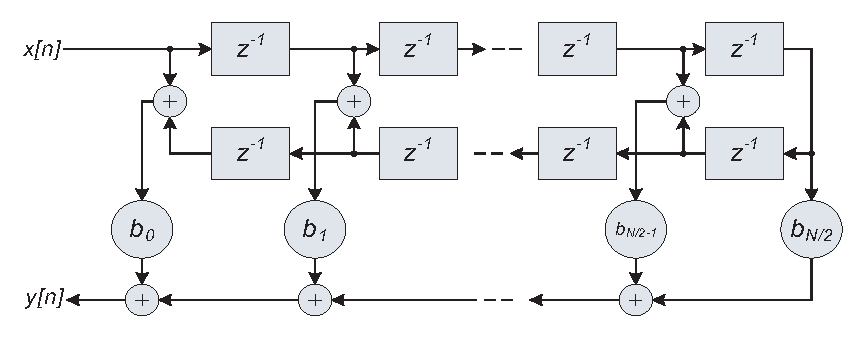
\includegraphics[width=13cm]{bilder/empfaenger/filter/FIRLinearphasenstruktur}
	\caption{Linearphasenstruktur eines FIR-Filters}
	\label{fig:FIRLinearphasenstruktur2}
\end{figure}

Hier wird auch deutlich, warum die Multiplizierer eine gr��ere Wortbreite aufweisen, als die �blicherweise verwendeten Wortbreiten (8,16,32). Durch die Addition zweier Zahlen vor dem Multiplizierer, erh�ht sich die Wortbreite dieser Zahl um ein Bit, wenn man gleiche Genauigkeit voraussetzt (vgl. \ref{subsec:siggen:machinenumbers}). Bei der Addition zweier Zahlen beispielsweise die nahe an den Grenzen des darstellbaren Bereichs liegen (z.B. $0,9 + 0,8 = 1,7$) wird der Wertebereich der Eingangsvariablen $[-1;1[$ verlassen. Indem ein weiteres Bit vor dem Komma zur Verf�gung gestellt wird, das bei Addierern "`Carry-Bit"' genannt wird, umgeht man diese Einschr�nkung und kann dem Multiplizierer eine Zahl mit m�glichst hoher Genauigkeit zuf�hren. Anschlie�end muss die Genauigkeit des Ergebnisses beschnitten werden, um eine Weiterverarbeitung zu erm�glichen.

\paragraph{Aufgabe 1:}

Programmieren sie das Filter mit der Ordnung $N$ mit Hilfe von $\frac{N}{2}$ Multiplizierern aus dem sysDSP-Block in \verb|07_Bandpass\bandpass.vhd| und testen sie dies mit dem verschiedenen Frequenzen in und ausserhalb des Durchlassbereichs.
